\documentclass[withoutpreface,bwprint]{cumcmthesis} %去掉封面与编号页
\usepackage[final]{pdfpages}
\title{《软件需求工程 B》 大作业课题}
\tihao{A}

\baominghao{4321}
\schoolname{武汉理工大学}
\membera{小米}
\memberb{向左}
\memberc{哈哈}
\supervisor{老师}
\yearinput{2017}
\monthinput{08}
\dayinput{22}

% 添加pdf封面
\usepackage[final]{pdfpages}



% \begin{enumerate}[itemindent=1em]  %在这里设置缩进的距离
%     \item 将信号量S的值减1,即进行S = S-1;   
% \end{enumerate}

% \newpage
% % 代码附录
% \begin{appendices}
% \section{爬取店铺POI}
% \begin{lstlisting}[language=python]
%  \end{lstlisting}
% \section{评论数据爬取}
% \begin{lstlisting}[language=python]
% \end{lstlisting}
% \end{appendices}

\begin{document}

\includepdf{class_head.pdf}
\newpage
% \maketitle
%  \begin{abstract}
 
% \keywords{\TeX{}\quad  图片\quad   表格\quad  公式}
% \end{abstract}
% 
\includepdf[pages={1,2}]{head.pdf} 
% \newpage
% 目录
% \tableofcontents

\newpage

\section*{\LARGE 彩色图像修复问题}


\section{问题背景}
Sergei Mikhailovich Prokudin-Gorskii (1863 - 1944)是一位超越其所在时代的人,早在1907年,他就坚信彩色摄影将成为未来的发展趋势。在当时,由于沙皇的特别许可,他可以周游辽阔的沙俄帝国并拍摄他所看到的事物,包括列夫·托尔斯泰唯一的彩色肖像。他用简单原始的彩色摄影法拍下了很多东西:人、建筑、风景、铁路、桥梁……!

其所采用的彩色摄影法很简单:分别用红、绿、蓝滤光片把每个场景的三次曝光记录到一个玻璃底板上,并设想通过特殊的投影装置将三种颜色的底片叠加显示,从而让观众能够通过彩色照片了解这个幅员辽阔的国家。可惜,他的计划从未实现:他在1918年的十月革命后离开了俄罗斯,再也没有回来。幸运的是,他所拍摄的沙俄帝国最后几年的RGB玻璃板底片保存了下来,并于1948年被美国国会图书馆(LoC)买下。LoC最近将底片数字化,并可以通过网络供公众下载。

\section{问题描述}
利用图像处理技术,基于数字化存储的玻璃底板图像自动生成尽量非虚化的彩色图像。为完成本次实验,你需要从原始图像文件中分割提取三个彩色通道图像,将它们对齐并彼此叠加在一起,最终形成一张RGB彩色图像。

美国国会图书馆在其网站上详细说明了他们对这批照片进行复原并创建彩色图像的过程,
可以参考 http://www.loc.gov/exhibits/empire/making.html。

\section{问题分析及设计思路}
为了重新修复这些照片,我们需要尽量对齐三长分开的红色,绿色和蓝色通道的图像(简称为R,G,B通道)。
下面是我的主要方法:
\begin{enumerate}[itemindent=2em]  %在这里设置缩进的距离
    \item 只需将每张图片的高度 height / 3用作每个通道的高度,即可将原始图像裁剪为三个单独的通道图像。
    \item 以一定比例裁剪每个通道的边缘。这样做是为了算法可以在对齐时主要考虑图像的内部,而边框和其他瑕疵不会影响任何计算。
    \item 将裁剪后的红色和绿色通道与蓝色通道对齐,以获取两个通道的(x,y)位移。
    \item 将位移应用于每个通道的未裁剪图像,根据重叠部分进行重新裁剪,以保留尽可能多的图像。
    \item 将三个通道合并为一个最终图像并保存。
\end{enumerate}

\section{解决方案及结果分析}

\subsection{构造图像相似性矩阵}

现阶段有许多图像对齐方法,其中较为简单的方法是另R和G通道分别与B通道在任意的x、y移位范围内进行比较。我选择使用31 * 31的搜索块(左、右、上、下移动15个像素),计算图像中最小搜素块之间的最小均方误差即为合适移动量。
下面是两个比较算法:
\subsubsection*{Sum of Squared Differences (SSD)}
$ssd = sum( sum( (image1 - image2) ^ 2 ) )$
\begin{lstlisting}[language=python]
def SSD(im1, im2):
	try:
		return -np.linalg.norm(np.abs(np.gradient(im1)[0]) - np.abs(np.gradient(im2)[0])) - np.linalg.norm(np.abs(np.gradient(im1)[1]) - np.abs(np.gradient(im2)[1]))
	except ValueError:
		return -np.linalg.norm(im1 - im2)
\end{lstlisting}



以image1图像的源匹配点为中心,定义一个窗口D,其大小为$(2m+1)(2n+1)$,统计其窗口的灰度值的和,
然后在image2图像中逐步计算其左右窗口的灰度和的差值,最后搜索到的差值最小的区域的中心像素即为匹配点。
\subsubsection*{Normalized Cross Correlation (NCC)}
$ncc = innerproduct( image1 / ||image1||, image2 / ||image2|| )$
\begin{lstlisting}[language=python]
def NCC(im1, im2, eps=1e-7):
	try:
		grad1, grad2 = np.gradient(im1), np.gradient(im2)
		l = grad1[0].size
		grad1x, grad2x = grad1[0].reshape((l, )), grad2[0].reshape((l, ))
		grad1y, grad2y = grad1[1].reshape((l, )), grad2[1].reshape((l, ))
		grad1x, grad2x = grad1x / (np.linalg.norm(grad1x) + eps), grad2x / (np.linalg.norm(grad2x) + eps)
		grad1y, grad2y = grad1y / (np.linalg.norm(grad1y) + eps), grad2y / (np.linalg.norm(grad2y) + eps)
        return np.abs(grad1x).dot(np.abs(grad2x)) + np.abs(grad1y).dot(np.abs(grad2y))
    except ValueError:
		im1, im2 = im1.reshape((im1.size, )), im2.reshape((im2.size, ))
		im1_normalized, im2_normalized = im1 / np.linalg.norm(im1), im2 / np.linalg.norm(im2)
		return im1_normalized.dot(im2_normalized)
    \end{lstlisting}

NCC将平移后的图像进行归一化,然后将图像image1与被比较图像image2的内积作为矢量。这个值越大,两个图像位置
就越接近。


\subsection{结果分析}
\begin{figure}[H]
    \centering
    \begin{minipage}[c]{0.3\textwidth}
        \centering
        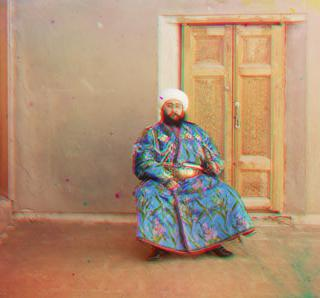
\includegraphics[width=0.95\textwidth]{000153v}
        \label{fig:sample-figure-a}
    \end{minipage}
    \begin{minipage}[c]{0.3\textwidth}
        \centering
        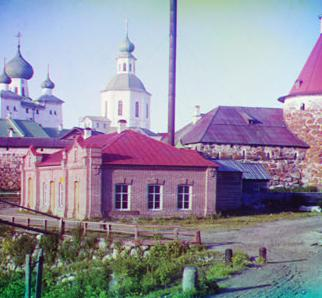
\includegraphics[width=0.95\textwidth]{000351v}
        \label{fig:sample-figure-b}
    \end{minipage}
    \begin{minipage}[c]{0.3\textwidth}
        \centering
        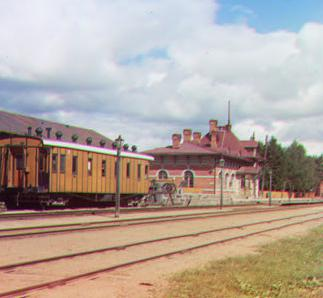
\includegraphics[width=0.95\textwidth]{000398v}
        \label{fig:sample-figure-c}
    \end{minipage}

    \begin{minipage}[c]{0.3\textwidth}
        \centering
        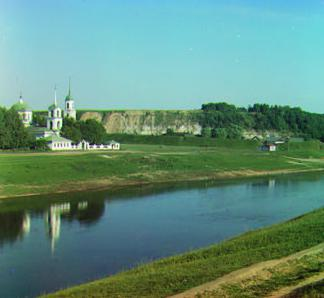
\includegraphics[width=0.95\textwidth]{000125v}

        \label{fig:sample-figure-a}
    \end{minipage}
    \begin{minipage}[c]{0.3\textwidth}
        \centering
        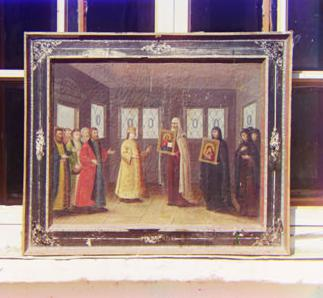
\includegraphics[width=0.95\textwidth]{000149v}
  
        \label{fig:sample-figure-b}
    \end{minipage}
    \begin{minipage}[c]{0.3\textwidth}
        \centering
        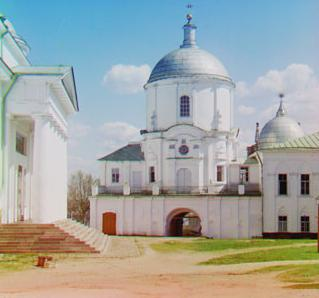
\includegraphics[width=0.95\textwidth]{001112v}

        \label{fig:sample-figure-c}
    \end{minipage}
    \caption{多图并排示例}
    \label{fig:sample-figure}
\end{figure}


尽管两种方法得到的结果相同,但SSD的计算速度比NCC略快,SSD在大约3秒内完成校准,NCC在大约6秒内完成校准。
\begin{table}[!htbp]
    \caption{jpg图像算法时间消耗}\label{tab:002} \centering
    \begin{tabular}{ccccc}
        \toprule[1.5pt]
        images & SSD /s   & NCC /s\\
        \midrule[1pt]
        cathedral.jpg& 2.64537906647  &	5.76754999161\\
        monastery.jpg& 3.01922702789& 	5.31478595734 \\
        nativity.jpg& 3.13875508308 &	5.24833297729 \\
        settlers.jpg& 2.9219288826 &	5.18062806129 \\
        tobolsk.jpg& 2.94660711288 &	6.85429000854 \\
        \bottomrule[1.5pt]
    \end{tabular}
\end{table}

\section{优化方案及对比}

\subsection{基于边缘的改进}
在较小的图像中,直接在颜色通道的特征空间上计算时间复杂度还可以接受。 但是,对于较大的图像,不仅遍历较多,还会因为通道之间的强度值急剧不同,导致时间消耗较大。

不仅如此,将SSD方法直接应用于彩色通道,尤其是较大的图像,由于这些通道之间的强度值不同,只会产生较差的对齐位移。 因此,颜色通道会通过边缘检测滤镜(skimage中的filters),以生成隔离图像边缘的二进制图像。

这在比较算法中用作预处理步骤,然后在这些二进制图像上使用SSD方法。 这里的相似性度量产生更好的结果,因为两个二进制图像的匹配误差百分比较低。 部分原因是由于边缘孤立的二进制图像消除了强度的大偏差。

对于特定类型的滤镜,大多数情况下使用Roberts算子,因为它可以近似图像中的梯度,从而节省了计算时间。 但是,在没有明显渐变的较平滑图像上,改用Canny算子,因为它使用高斯滤波的导数来计算渐变。
下面是未经过完全裁剪的图片:
\begin{figure}[H]
	\centering
	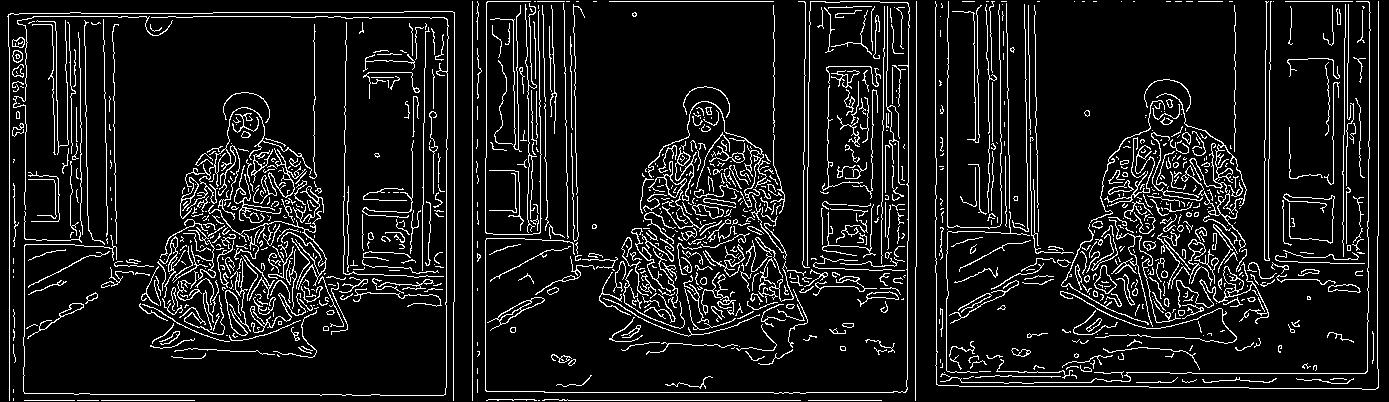
\includegraphics[width=16cm]{emir-edge.jpg}
    \caption{ sobel边缘 - emir.jpg \label{fig:1}}
\end{figure}

\begin{figure}[H]
	\centering
	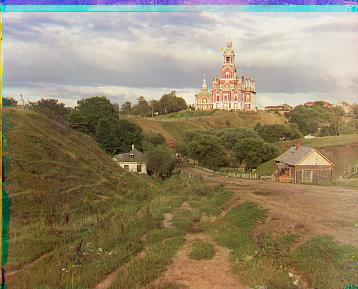
\includegraphics[width=12cm]{merged_cathedral.jpg}
    \caption{ sobel,canny边缘对齐运行结果 - cathedral.jpg \label{fig:1}}
    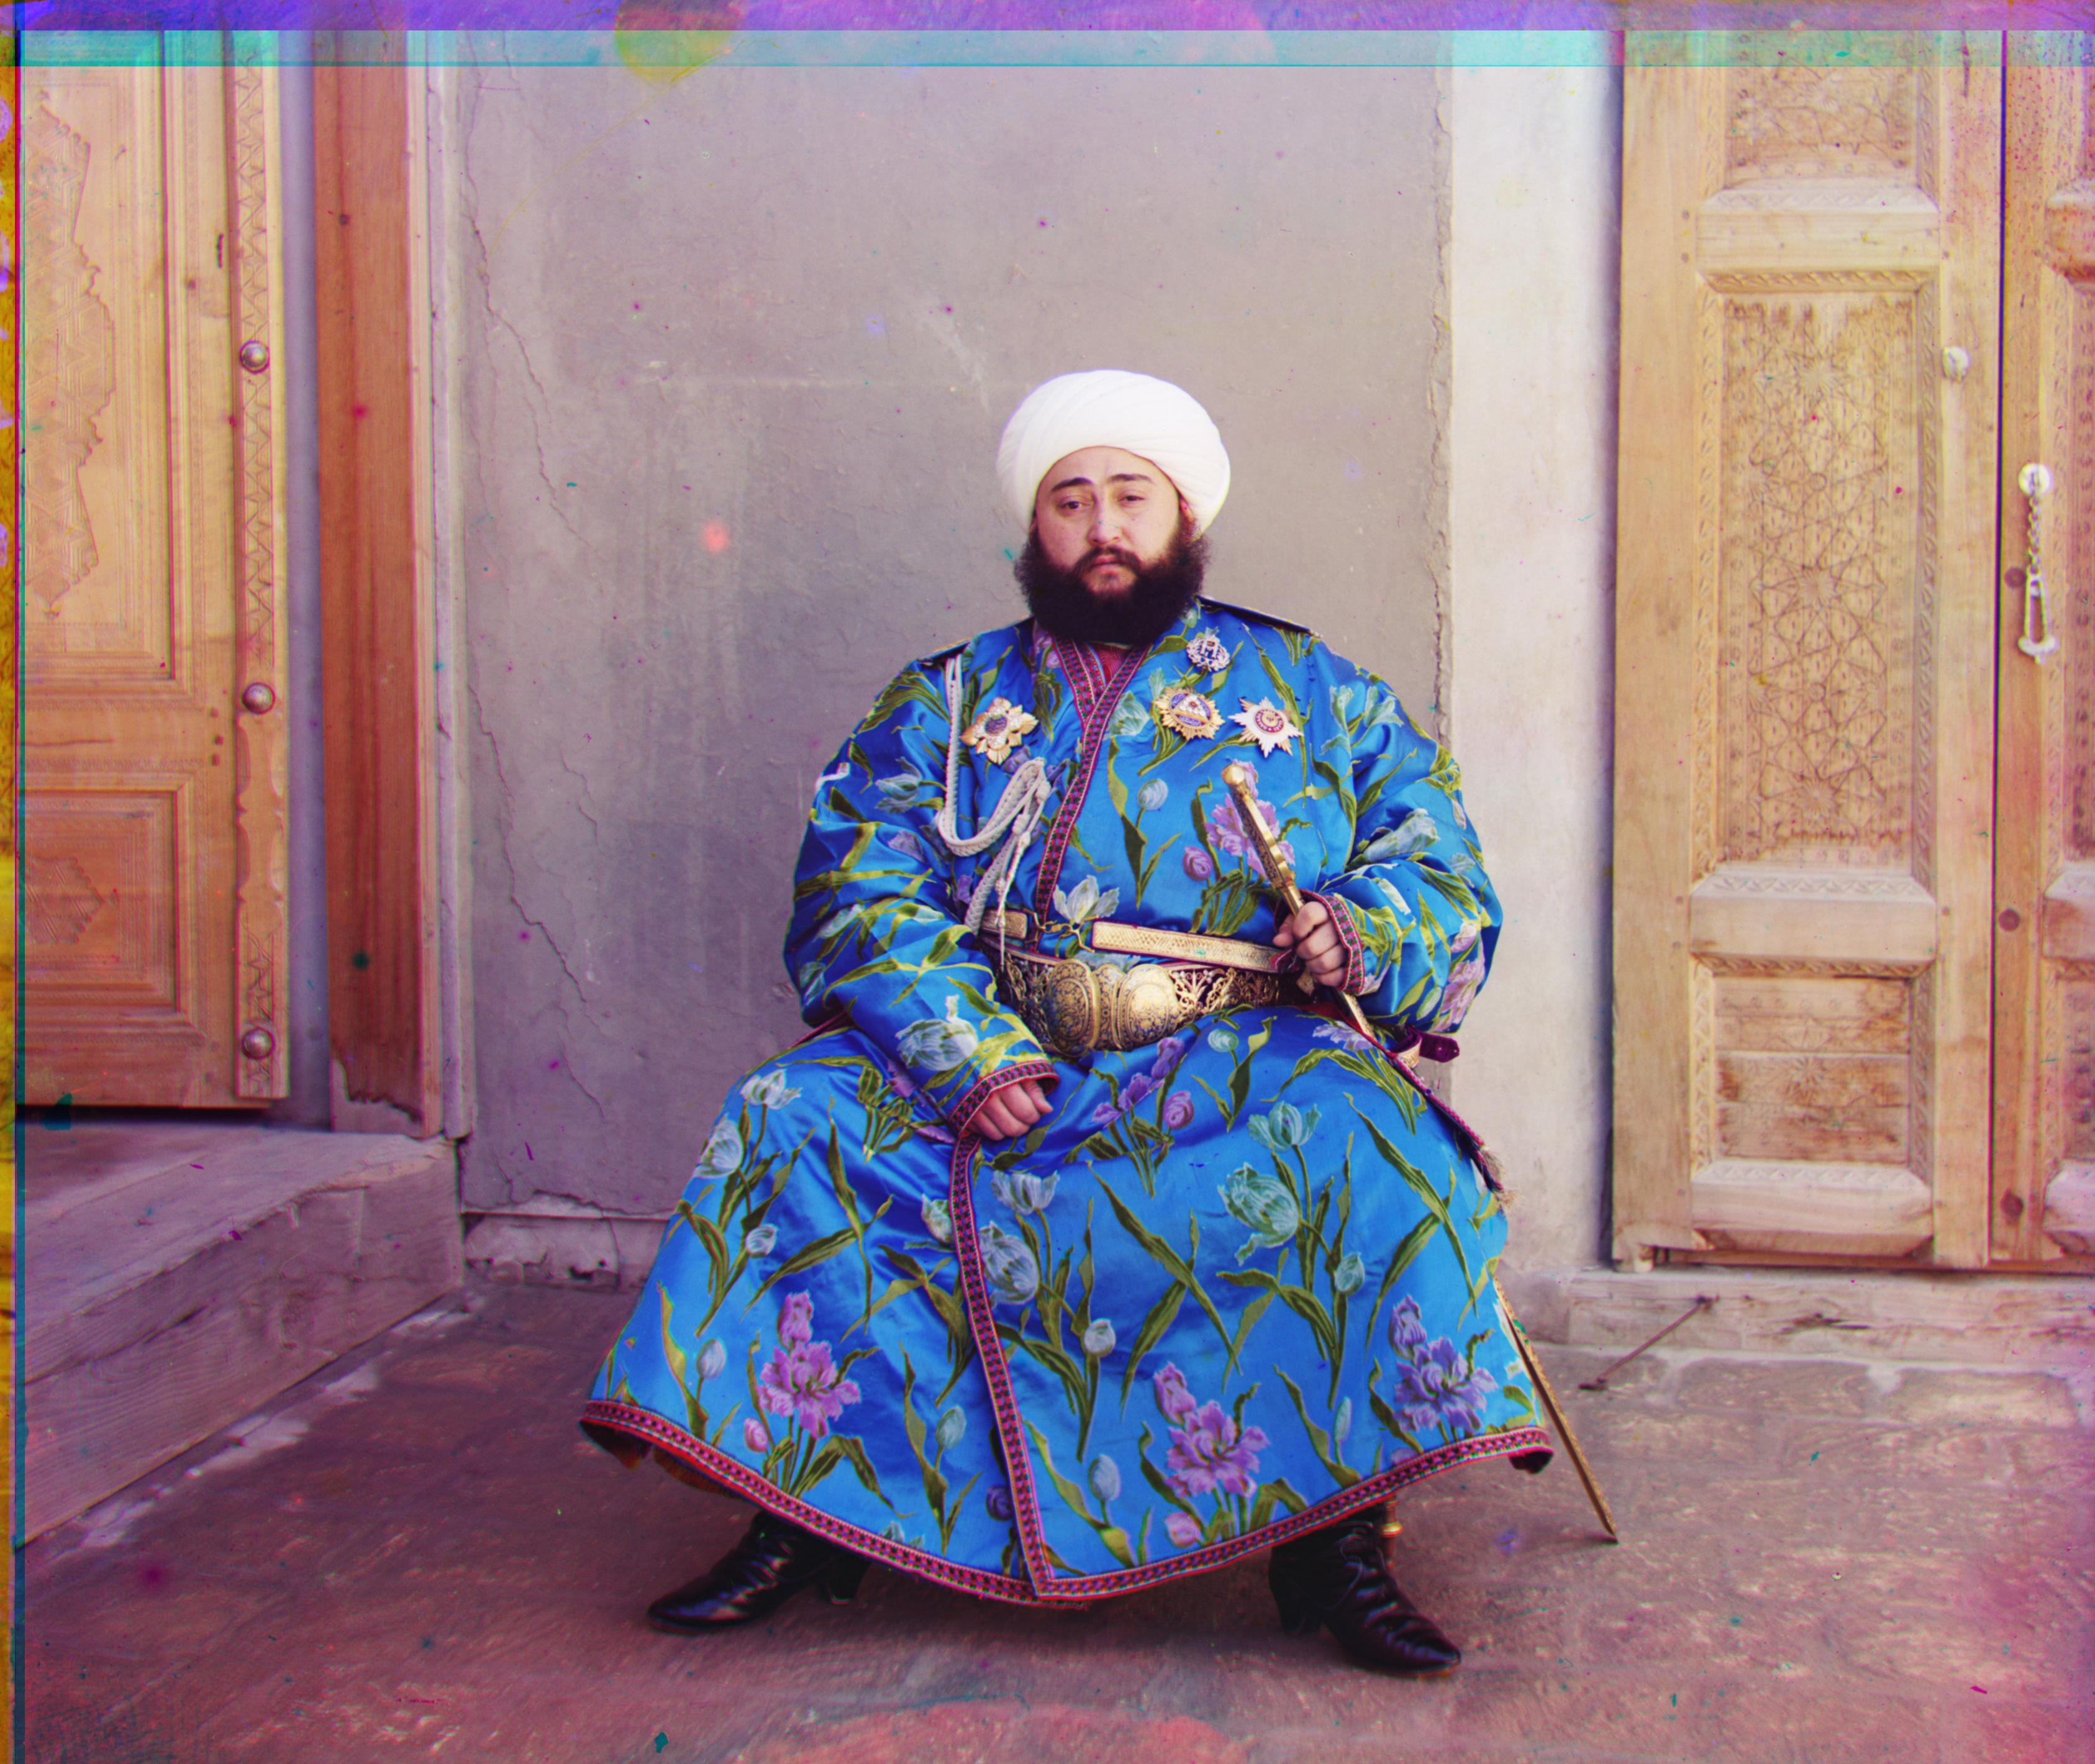
\includegraphics[width=12cm]{merged_emir.jpg}
	\caption{ sobel,canny边缘对齐运行结果 - emir.tif \label{fig:1}}
\end{figure}
\begin{table}[!htbp]
    \caption{tif图像算法时间消耗}\label{tab:003} \centering
    \begin{tabular}{ccccc}
        \toprule[1.5pt]
        images &SSD	/s & NCC /s \\
        \midrule[1pt]
        bridge.tif&	13.7140870094 &	14.0207099915 \\
        harvesters.tif&	18.6445329189 &	20.7564790249 \\
        lady.tif&	15.0626921654 &	19.761646986 \\
        melons.tif&	21.7461268902 &	20.1103210449 \\
        onion\_church.tif &	20.0455958843 &	22.6522738934  \\
        self\_portrait.tif &	17.4606361389 &	32.0704319477  \\
        three\_generations.tif &	13.7146379948 &	17.5942869186 \\
        turkmen.tif & 17.5983920097 &	15.437732935 \\
        workshop.tif&	17.8079559803 &	21.5742030144 \\
        \bottomrule[1.5pt]
    \end{tabular}
\end{table}

\section{进一步的改进方向}

本次实验还有很多未实现的思考,比如调整对比度:在合成彩色图片前,对图像的亮度进行重新标定是常用的处理手法。例如,在平均亮度最暗的颜色通道上,其最黑的像素应被标定为0,在平均亮度最亮的颜色通道上,其最亮的像素应被标定为1(对8位图像而言,即255)。重新标定各个通道的亮度后,合成结果可能会有更好的质量。
;更好的颜色映射:由于老旧的摄影设备的误差,我们并不能断定拍摄原始图像时所用的红色、绿色和蓝色镜头准确对应于RGB颜色空间中的R、G和B通道。可尝试找到一个能产生更真实颜色的映射。


% \newpage
% % 代码附录
\begin{appendices}
\section{实验结果}

\section{彩色图像修复}
\begin{lstlisting}[language=python]
    import numpy as np
    import skimage as sk
    import skimage.io as skio
    import skimage.transform
    import skimage.filters
    from skimage import feature,data,color
    
    # name of the input file
    imname = 'emir.tif'
    #imname = 'cathedral.jpg'
    
    # read in the image
    im = skio.imread(imname)
    
    print("dimension: ", im.shape)
    # convert to double (might want to do this later on to save memory)    
    im = sk.img_as_float(im)
    
    # compute the height of each part (just 1/3 of total)
    height = im.shape[0] // 3
    width = im.shape[1]
    print("height: ", height)
    # separate color channels
    b = im[:height]
    g = im[height: 2*height]
    r = im[2*height: 3*height]
    
    canny = feature.canny(g) * 1
    diff = np.linalg.norm(canny - np.roll(canny, 1, axis=0), axis=0) / height
    print(canny[:10,:10])
    print(diff[450:460])
    print(np.mean(canny, axis=0)[450:460])
def SSD(im1, im2):
	try:
		return -np.linalg.norm(np.abs(np.gradient(im1)[0]) - np.abs(np.gradient(im2)[0])) - np.linalg.norm(np.abs(np.gradient(im1)[1]) - np.abs(np.gradient(im2)[1]))
	except ValueError:
		return -np.linalg.norm(im1 - im2)

def NCC(im1, im2, eps=1e-7):
	try:
		grad1, grad2 = np.gradient(im1), np.gradient(im2)
		l = grad1[0].size
		grad1x, grad2x = grad1[0].reshape((l, )), grad2[0].reshape((l, ))
		grad1y, grad2y = grad1[1].reshape((l, )), grad2[1].reshape((l, ))

		grad1x, grad2x = grad1x / (np.linalg.norm(grad1x) + eps), grad2x / (np.linalg.norm(grad2x) + eps)
		grad1y, grad2y = grad1y / (np.linalg.norm(grad1y) + eps), grad2y / (np.linalg.norm(grad2y) + eps)
		return np.abs(grad1x).dot(np.abs(grad2x)) + np.abs(grad1y).dot(np.abs(grad2y))
	except ValueError:
		im1, im2 = im1.reshape((im1.size, )), im2.reshape((im2.size, ))
		im1_normalized, im2_normalized = im1 / np.linalg.norm(im1), im2 / np.linalg.norm(im2)
		return im1_normalized.dot(im2_normalized)

    
def NCC2(arr1, arr2):
	arr1 = arr1.reshape((arr1.size, ))
	arr2 = arr2.reshape((arr2.size, ))
	return arr1.dot(arr2)

def pyramid_find_displacement(im, fixed, n, e, matching_metric=NCC):
	if n == 0:
		return find_displacement(im, fixed)
	im_resized = sk.transform.rescale(sk.filters.gaussian(im), .5)
	fixed_resized = sk.transform.rescale(sk.filters.gaussian(fixed), .5)
	displacement_vector = pyramid_find_displacement(im_resized, fixed_resized, n - 1, e * 2) * 2
	print("displacement vector: ", displacement_vector)
	print("shape: ", im.shape)
	return find_neighboring_displacement(im, fixed, displacement_vector, e, matching_metric)

def find_neighboring_displacement(im, fixed, displacement_vector, e, matching_metric=NCC):
	copy = np.copy(im)
	best_displacement_x = displacement_vector[0]
	best_displacement_y = displacement_vector[1]
	best_matching_score = float("-inf")
	h, w = im.shape
	x_lower_bound = max(best_displacement_x - e, -h//10 + 1)
	x_upper_bound = min(best_displacement_x + e, h//10 - 1) + 1
	y_lower_bound = max(best_displacement_y - e, -w//10 + 1)
	y_upper_bound = min(best_displacement_y + e, w//10 - 1) + 1
	for i in range(x_lower_bound, x_upper_bound):
		for j in range(y_lower_bound, y_upper_bound):
			im = np.roll(np.roll(copy, j, axis=1), i, axis=0)
			score = matching_metric(fixed, im)
			if score > best_matching_score:
				best_displacement_x, best_displacement_y, best_matching_score = i, j, score
			# print("\ti:{}, j, {}, x: [{}, {}], {}; y: [{},  {}], {}, score: {}, best score: {}".format(i, j, x_lower_bound, x_upper_bound, best_displacement_x, y_lower_bound, y_upper_bound, best_displacement_y, score, best_matching_score))

	return np.array([best_displacement_x, best_displacement_y])


def find_displacement(im, fixed, matching_metric=NCC):
	copy = np.copy(im)
	best_displacement_x = 0
	best_displacement_y = 0
	best_matching_score = float("-inf")
	h, w = im.shape
	for i in range(-h + 1, h):
		for j in range(-w + 1, w):
			im = np.roll(np.roll(copy, j, axis=1), i, axis=0)
			score = matching_metric(fixed, im)
			if score > best_matching_score:
				best_displacement_x, best_displacement_y, best_matching_score = i, j, score
	return np.array([best_displacement_x, best_displacement_y])

def pyramid_align(im, fixed, matching_metric=NCC):
	# skio.imshow_collection(np.gradient(im))
	# print(np.mean(np.gradient(im)[0]))
	# skio.show()
	n = int(np.floor(np.log2(np.min(im.shape))))
	displacement_x, displacement_y = pyramid_find_displacement(im, fixed, n, 1, matching_metric)
	print(displacement_x, displacement_y)
	return np.roll(np.roll(im, displacement_y, axis=1), displacement_x, axis=0)

def crop(r, g, b):
	for i in range(4):
		r, g, b = crop_one_side(r, g, b)
		r, g, b = np.rot90(r), np.rot90(g), np.rot90(b)
	return r, g, b
def crop_one_side(r, g, b):
	r_gradient, g_gradient, b_gradient = r, g, b

	row_to_crop = max(find_row_to_crop(r_gradient), find_row_to_crop(g_gradient), find_row_to_crop(b_gradient))
	print("row to crop: ", row_to_crop)
	r_cropped, g_cropped, b_cropped = r[:,row_to_crop:], g[:,row_to_crop:], b[:,row_to_crop:]

	return r_cropped, g_cropped, b_cropped

def find_row_to_crop(im, thresh=.90):
	m = 0
	_, w = im.shape
	end = w // 10
	canny = feature.canny(im) * 2 - 1
	h, _ = canny.shape
	left_width = 4
	line_width = 2
	right_width = 1
	mask_width = left_width + line_width + right_width
	mean = np.mean(canny, axis=1)
	mask = np.concatenate((-1 * np.ones((h, left_width)), np.ones((h, line_width)), -1 * np.ones((h, right_width))), axis=1)
	# mask = np.concatenate((-1 * np.ones((h, left_width)), np.ones((h, line_width)), -1 * np.ones((h, right_width))), axis=1)
	border = 0
	best_score = float("-inf")
	print(np.sum(canny[:, line_width + right_width]))
	print(canny.shape, im.shape)

	# print(canny[:20,:20])
	print(best_score)
	scores = []
	while (m < end):
		score = NCC2(mask, canny[:, m: m + mask_width])
		scores.append(score)
		if (score > best_score):
			best_score = score
			border = m + left_width
		print("best score: ", best_score, border, "score: ", score, m)
		m += 1
	scores = np.asarray(scores)
	std = np.std(scores)
	mean = np.mean(scores)
	print("sd: ", std, "mean: ", mean)
	local_maxima_indices = np.where(scores >= mean + std)[0]
	print("local maxima:", local_maxima_indices)
	if len(local_maxima_indices) > 0 and np.max(local_maxima_indices) + left_width > border:
		border = np.max(local_maxima_indices) + left_width
	return border

def find_row_to_crop_black(im, thresh=.2):
	start = 0
	h, w = im.shape
	end = w
	m = 0 #(start + end) // 2
	blocksize = 8
	while (m < w // 10):
		if np.mean(np.abs(im[:,m:m+8])) > thresh:
			if blocksize == 1:
				break
			else:
				blocksize -= 1
		else:
			m += blocksize
		print(m, np.mean(np.abs(im[:,m:m+blocksize])))
		m += blocksize
	return m

def difference_of_gaussians(im, num_differences=5):
	sigmas = np.linspace(0, 2, 2 * num_differences)
	difference = np.zeros(im.shape)
	for i in range(num_differences):
		sigma1 = sigmas[2*i]
		sigma2 = sigmas[2*i+1]
		difference += sk.filters.gaussian(im, sigma=sigma1) - sk.filters.gaussian(im, sigma=sigma2)
	return difference / num_differences * 100

def get_luminance(r, g, b):
	return  0.2126 * r + 0.7152 * g + 0.0722 * b

def get_brightest_pixel(channel):
	brightest_index = np.argmax(channel)
	h, w = channel.shape
	x, y = brightest_index // h, brightest_index % w
	return x, y

def get_darkest_pixel(channel):
	darkest_index = np.argmin(channel)
	h, w = channel.shape
	x, y = darkest_index // h, darkest_index % w
	return x, y

def auto_contrast(r, g, b):
	luminance = get_luminance(r, g, b)
	brightest_x, brightest_y = get_brightest_pixel(luminance)
	darkest_x, darkest_y = get_darkest_pixel(luminance)
	brightest_channel_index = np.argmax([r[brightest_x, brightest_y], 
										 g[brightest_x, brightest_y],
										 b[brightest_x, brightest_y]])
	print(brightest_channel_index)
	brightest_channel = [r, g, b][brightest_channel_index]
	darkest_channel_index = np.argmin([r[darkest_x, darkest_y], 
									g[darkest_x, darkest_y],
									b[darkest_x, darkest_y]])
	print(darkest_channel_index)
	darkest_channel = [r, g, b][darkest_channel_index]
	darkest_channel = normalize_brightness(darkest_channel)
	result = [r, g, b]
	result[brightest_channel_index] = normalize_brightness(brightest_channel)
	result[darkest_channel_index] = normalize_brightness(darkest_channel)
	return result
def normalize_brightness(channel):
	brightest_value = np.max(channel)
	darkest_value = np.min(channel)
	scale = brightest_value - darkest_value
    return (channel - darkest_value) / scale
r_cropped, g_cropped, b_cropped = crop(r, g, b)
ar = pyramid_align(r_cropped, b_cropped)
ag = pyramid_align(g_cropped, b_cropped)
# create a color image
im_stacked = np.dstack([r, g, b])
im_out = np.dstack([ar, ag, b_cropped])
im_manual = np.dstack([np.roll(np.roll(r, 120, axis=0), 8, axis=1), np.roll(np.roll(g, 50, axis=0), 30, axis=1), b])

# save the image
im_out = img_as_ubyte(im_out) # 将float64转化为uint8格式
fname = '../out_fname.jpg'
skio.imsave(fname, im_out)
print("cropped size: ", r_cropped.shape)
# display the image
# skio.imshow(im_out)
# skio.imshow_collection([ar, ag, b_cropped])
print(b_cropped[50,:50])
cr, cg, cb = auto_contrast(ar, ag, b_cropped)
print(cb[50,:50])
# skio.imshow_collection([np.gradient(r_cropped)[0] * 100, np.gradient(b_cropped)[0] * 100])
# skio.show()
# skio.imshow_collection([im_stacked, im_out])
skio.imshow_collection([im_out, np.dstack([cr, cg, cb])])
# skio.imshow_collection([r_cropped, g_cropped, b_cropped, im_out])
skio.show()
\end{lstlisting}
\end{appendices}
% %参考文献
% \begin{thebibliography}{9}%宽度9
%     \bibitem[1]{1}
%     李洁, 张瑜慧. 信号量在生产者-消费者及其变形问题中的应用[J]. 福建电脑, 2012(02):175-177.
%     \bibitem[2]{2}
%     李志民, 赵一丁, 底恒. 操作系统进程同步的教学实践[C]// 计算机研究新进展(2010)——河南省计算机学会2010年学术年会论文集. 2010.步的教学实践[C]计算机研究新进展(2010)——河南省计算机学会2010年学术年会论文集. 2010.
%     \bibitem[3]{3}
%     陈涛,任海兰. 基于Linux的多线程池并发Web服务器设计[J]. 电子设计工程, 2015(11):175-177.
%     \bibitem[4]{4}
%     李盼盼, 赵浩. 基于信号量机制的生产者消费者问题的分析[J]. 无线互联科技, 2013(11):101-102.
% \end{thebibliography}

\end{document}
